\preparagraphspacing{}
\section*{Change Descriptors}
\label{sec:chdescs}

{\bf This section refers to LFS before it is defined.}

In contrast with traditional systems, where changes to filesystem data are
accomplished by changing in-memory copies of the disk blocks and marking the
block as needing to be written to disk (thus losing all record of what was
changed), every change to filesystem data in the KudOS file server effects a
corresponding ``change descriptor'' that describes what was changed. Change
descriptors (``chdescs'' for short) allow a dependency graph to be created
describing which changes depend on which other changes already being written to
disk, as well as allowing individual changes to be undone and redone. These two
capabilities allow any module in the system to inspect and even modify the
changes that other modules are making.

The ability to revert and re-apply chdescs is inspired by the ``soft updates''
system in BSD's FFS~\cite{ganger00soft}, but it is generalized so that it is not
specific to any particular filesystem. A chdesc can describe a change as small
as a single bit, or as large as a whole disk block. Soft updates, journalling,
and many application-specific consistency models all correspond to different
change descriptor arrangements. Block data is almost secondary to the chdescs
from the point of view of the file system server -- chdescs are what really move
around in the system. This concept allows some interesting configurations of
modules as well as very simple implementations of traditionally complicated
features. For instance, journalling is implemented as a single block device
module, and it can automatically add journalling -- even metadata-only
journalling -- to {\it any} LFS filesystem. Other block device layering systems,
like GEOM~\cite{geom}, would need special hooks into filesystem code in order to
get the necessary hints (i.e. what is metadata and what is not) to do
metadata-only journalling. Change descriptors and the LFS interface division
allow us to do this automatically.

For many complex operations, like RAID or journalling, the chdesc graph is
changed in specific ways which can be broken down into sequences of simple graph
transformations. For example, in the (mirroring) RAID module it is necessary to
duplicate a change descriptor, including all its dependents and dependencies. We
expect that after implementing a relatively small number of more complex modules
(we have only implemented the two mentioned), we will have seen similarities in
many of the transformations and will have built up a fairly complete library of
common transformation functions.

\begin{figure}
\begin{verbatim}
struct chdesc {
    BD_t * owner;
    bdesc_t * block;
    enum {BIT, BYTE, NOOP} type;
    union {
        struct {
            uint16_t offset;
            uint32_t xor;
        } bit;
        struct {
            uint16_t offset, length;
            uint8_t * data;
        } byte;
    };
    struct chdesc * dependencies[];
};
\end{verbatim}
\caption{\label{fig:chdesc} Change descriptor structure}
\end{figure}

\begin{figure}
  \centering
  \includegraphics[width=\columnwidth]{fig/whatevs_2}
  \caption{\label{fig:journal} Journal}
\end{figure}

\begin{figure}
  \centering
  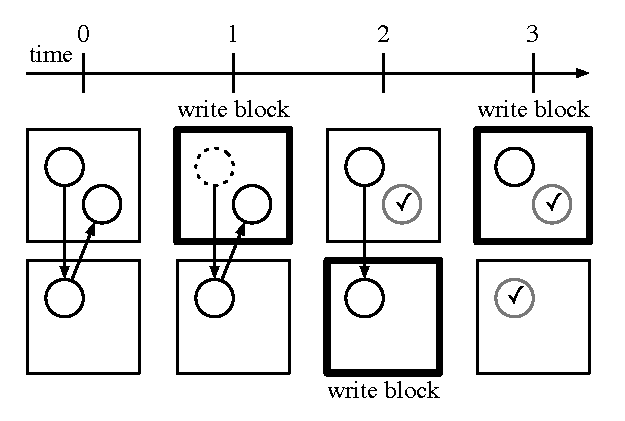
\includegraphics[width=\columnwidth]{rollback_sequence}
  \caption{\label{fig:rollback} Rollback}
\end{figure}
